\documentclass[11pt,a4paper]{article}

% ================== Packages ==================
\usepackage[utf8]{inputenc}
\usepackage[T1]{fontenc}
\usepackage[french]{babel}
\usepackage{lmodern}
\usepackage{geometry}
\usepackage{float}
\geometry{hmargin=2cm, vmargin=2cm}
\usepackage[bottom]{footmisc}
\usepackage{amsmath, amssymb}
\usepackage{graphicx}
\usepackage{placeins}
\usepackage{hyperref}
\usepackage{enumitem}
\usepackage{setspace}
\usepackage{titlesec}
\usepackage{subcaption}

\setstretch{1.2}

% ================== Title formatting ==================
\titleformat{\section}{\large\bfseries}{\thesection}{1em}{}
\titleformat{\subsection}{\normalsize\bfseries}{\thesubsection}{1em}{}

% ================== Document ==================
\begin{document}

\begin{titlepage}
\centering

% Logo de l'université au milieu/haut
\includegraphics[width=0.4\textwidth]{logo-ub.png}\\[1cm] 

{\LARGE \textbf{Projet de Programmation}}\\[0.3cm]
{\Large Master Informatique 2025--2026}\\[1.5cm]

{\Huge \textbf{Rapport préliminaire}}\\[0.3cm]
{\Large Analyse des besoins du projet \textit{Dames}}\\[1.5cm]

\vfill

\begin{minipage}{0.8\textwidth}
\centering
\textbf{Préparé par :}\\[0.2cm]
Fy-Tommy RAMANANAHERISOA \\
Faniry HOAREAU \\
Lalatiana RANDRIAMIHAJA \\
Daniel ATWI \\
Sarah RAZAFINDRAKOTO
\end{minipage}

\vfill

\textbf{Université de Bordeaux}\\[0.5cm]
29 Janvier 2026 

\end{titlepage}

\tableofcontents
\newpage

% ======================================================
\section{Contexte et objectifs du projet}

Le projet a pour objectif de concevoir et développer un logiciel permettant de jouer au jeu de dames conformément aux règles officielles. Le programme doit permettre à deux joueurs de s’affronter sur un damier, soit en mode local, soit à distance via un réseau.

Le jeu de dames est un jeu déterministe à information parfaite. Le logiciel doit garantir le respect strict des règles du jeu tout en proposant une expérience utilisateur claire, robuste et extensible. Le projet s’inscrit dans une démarche de développement logiciel complète intégrant la qualité du code \footnote{Les bonnes pratiques d'implémentation suivent les recommandations de Joshua Bloch, \textit{Effective Java}, 3rd Edition, 2017.}, la documentation, les tests \footnote{Méthodologie basée sur M. Aniche, \textit{Effective Software Testing: A Developer's Guide}, Manning, 2022.} et les performances.

\subsection{Historique}

Le jeu de dames puise ses origines dans l'Alquerque, un jeu déterministe apparu vers le VIIème siècle en Afrique du Nord avant de se diffuser via l'Espagne. Historiquement, le jeu est littéralement « gravé dans l'histoire », comme en témoignent les diagrammes retrouvés sur des dalles de temples antiques. Au Moyen Âge, la transition s'opère sur l'échiquier bicolore ; c'est d'ailleurs dans les enluminures médiévales représentant la noblesse que le nom « Jeu de Dames » trouve sa source.

\subsection{Règles et but du Jeu}

Le jeu de dames se décline en de nombreuses variantes internationales que notre programme doit pouvoir supporter via l'option --size. Parmi les plus notables, on compte le style anglo-saxon (Draughts) sur un damier de 8x8, le standard international sur un plateau de 10x10, et les dames canadiennes s'affrontant sur une grille de 12x12. Le logiciel doit ainsi être capable d'adapter sa logique de jeu à ces différentes dimensions de plateau.

Le programme implémente les règles officielles du jeu de dames \footnote{Règles consultées sur : \url{https://www.ffjd.fr/Web/index.php?page=reglesdujeu}}
, validées par le serveur pour garantir l'intégrité de chaque partie. Sur un damier orienté avec une case sombre en bas à gauche , le jeu se pratique exclusivement sur les cases foncées où, en configuration 10x10, chaque joueur dispose de 20 pions répartis sur les quatre premières rangées. Les blancs engagent la partie et les joueurs alternent leurs tours. Le pion progresse d'une case en diagonale vers l'avant, tandis que la promotion en « dame » sur la dernière rangée lui offre une liberté de mouvement totale sur ses diagonales. La victoire est acquise par la capture de l’intégralité des pièces adverses ou par l'immobilisation totale du joueur adverse.

\subsection{La prise par un pion}

La capture d'un pion s'effectue par un saut au-dessus de la pièce adverse vers une case libre située immédiatement derrière, entraînant son retrait définitif du plateau. Cette manœuvre est obligatoire et peut être réalisée aussi bien vers l'avant que vers l'arrière. Si l'état du jeu le permet, les prises doivent être enchaînées en une seule séquence continue jusqu'à épuisement des captures possibles. Conformément aux règles officielles, l'ensemble des pièces capturées n'est retiré du damier qu'à l'issue complète de la rafle.

\subsection{La prise majoritaire}

Cette règle, dite de la prise majoritaire, impose de privilégier le chemin de capture offrant le plus grand nombre de pièces, quel que soit leur rang. Ainsi, une séquence permettant de capturer deux pions est prioritaire sur la prise d'une dame isolée.

Dans la Figure \ref{fig:prise-majoritaire}, un pion blanc peut prendre un pion noir, mais l'autre pion blanc peut en prendre 3, c'est donc ce coup qui doit être joué.

\subsection{La prise par la dame}

Grâce à son amplitude de mouvement, la dame dispose de capacités de capture étendues. Elle doit capturer toute pièce située sur ses diagonales dès lors qu'une case libre est disponible immédiatement derrière. S'il est interdit de franchir plus d'une fois le même pion au cours d'une séquence, le passage multiple par une même case vide est autorisé.

Dans la Figure \ref{fig:prise-dame}, la dame blanche peut prendre les 4 pions noirs et pourra s'arrêter au choix sur l'une des 2 cases marquées d'une croix.

\begin{figure}[htbp]
     \centering
     % --- Première image ---
     \begin{subfigure}[b]{0.3\textwidth}
         \centering
         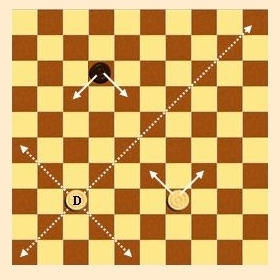
\includegraphics[width=\textwidth]{diagdam2.jpg}
         \caption{La prise de pion}
         \label{fig:prise-pion}
     \end{subfigure}
     \hfill
     % --- Deuxième image ---
     \begin{subfigure}[b]{0.3\textwidth}
         \centering
         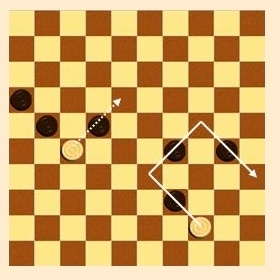
\includegraphics[width=\textwidth]{diagdam3.jpg}
         \caption{La prise majoritaire}
         \label{fig:prise-majoritaire}
     \end{subfigure}
     \hfill
     % --- Troisième image ---
     \begin{subfigure}[b]{0.3\textwidth}
         \centering
         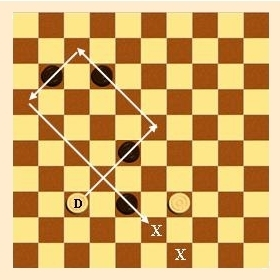
\includegraphics[width=\textwidth]{diagdam4.jpg}
         \caption{La prise par la dame}
         \label{fig:prise-dame}
     \end{subfigure}
     
     \caption{Mécaniques de capture du jeu de dames}
     \label{fig:prises}
\end{figure}

Enfin, la partie peut être déclarée nulle si aucun des deux joueurs ne peut prendre toutes les pièces adverses (par exemple 3 dames contre une).

\subsection{Versions existantes}

Dans le cadre de notre phase d'analyse, nous avons étudié le projet open-source \textbf{AwsDame}, une plateforme de jeu de dames multijoueur en temps réel. Bien que ce projet soit développé dans un environnement technique différent du nôtre (JavaScript/Node.js), son architecture offre des points de comparaison pertinents pour nos futurs développements, notamment pour la partie réseau.

Lien Github : \url{https://github.com/mortexsa/AwsDame}\\


\noindent Nous avons également étudié le logiciel \textbf{Raven Checkers}, un programme de dames open-source conçu principalement à des fins pédagogiques pour l'étude du jeu et des algorithmes d'intelligence artificielle. Il couple la fonction d'évaluation de \textit{Simple Checkers}
\footnote{Voir \url{https://www.fierz.ch/engines.php}} aux algorithmes de recherche du projet AIMA. \footnote{Peter Norvig's search code from the AIMA project : \url{http://aima.cs.berkeley.edu/python/readme.html}}

Dépôt : \url{https://github.com/bcorfman/raven-checkers}

\section{Complexité du jeu de Dames}

Le but de cette section est de chiffrer l'espace d'état du jeu et la complexité inhérente à ses règles, sans la confondre avec la complexité des algorithmes de recherche employés. Une telle analyse est indispensable pour justifier nos choix de structures de données et de méthodes de recherche.

\subsection{Analyse de l'espace d'états}

L'espace d'états (State-space complexity) représente le nombre de configurations légales du plateau. Ce nombre croît de manière exponentielle avec la taille du tablier :

\begin{itemize}
    \item \textbf{Dames 8x8 (Anglaises/Brésiliennes)} : Avec 32 cases actives, l'espace d'états est de $5 \times 10^{20}$ positions. Cette variante a été résolue par le programme Chinook en 2007, prouvant qu'une partie parfaite mène à la nulle \footnote{J. Schaeffer et al., \textit{Checkers Is Solved}, Science, Vol. 317, 2007.}.
    \item \textbf{Dames 10x10 (Internationales)} : Le passage à 50 cases actives fait grimper l'espace à environ $10^{30}$ positions. La complexité de l'arbre de jeu atteint environ $10^{54}$.
    \item \textbf{Dames 12x12 (Canadiennes)} : Avec 72 cases actives, l'espace d'états dépasse $10^{40}$, rendant toute tentative de résolution exhaustive informatiquement impossible avec les ressources actuelles.
\end{itemize}



\subsection{Approche algorithmique face à l'explosion combinatoire}

Face à ces chiffres, l'exploration exhaustive de l'arbre de jeu est impossible. Notre architecture logicielle implémente donc plusieurs stratégies pour naviguer dans cette complexité:

\begin{itemize}
    \item \textbf{Optimisation par Bitboards :} L'utilisation de types \texttt{long} (64 bits) pour représenter les pièces sur des plateaux 8x8 et 10x10 (nécessitant deux \texttt{long} pour 12x12) permet de calculer les coups légaux via des opérations bit à bit\footnote{Chess Programming Wiki, \textit{Bitboards}: \url{https://www.chessprogramming.org/Bitboards}}. Cela réduit le coût computationnel à chaque nœud de l'arbre.
    \item \textbf{Évaluation par Heuristique} : Puisque nous ne pouvons pas atteindre les feuilles de l'arbre (durée moyenne d'une partie de 80 à 100 demi-coups), nous utilisons la fonction \texttt{boardValue()} pour estimer la qualité d'une position.
\end{itemize}


% ======================================================
\section{Structure de données et algorithmes}

\subsection{Bitboard}


\subsubsection{Cases jouables}

Sur les \(100\) cases du plateau, seules les cases noires sont
utilisées pour le déplacement des pions.
Ainsi, seulement la moitié des cases est pertinente pour la
représentation de l'état du jeu.

\[
\text{Nombre de cases jouables} = \frac{Nombre de case total}{2} = 50 \text{ si le nombre de case est \(10\) x \(10\)}
\]

\subsubsection{Numérotation des cases}

Afin de simplifier la représentation interne du plateau, les
50 cases noires sont numérotées de \(0\) à \(49\), ligne par
ligne, de bas en haut et de gauche à droite.

\[
\begin{array}{cccccccccc}
\cdot & 45 & \cdot & 46 & \cdot & 47 & \cdot & 48 & \cdot & 49 \\
40 & \cdot & 41 & \cdot & 42 & \cdot & 43 & \cdot & 44 & \cdot \\
\cdot & 35 & \cdot & 36 & \cdot & 37 & \cdot & 38 & \cdot & 39 \\
30 & \cdot & 31 & \cdot & 32 & \cdot & 33 & \cdot & 34 & \cdot \\
\cdot & 25 & \cdot & 26 & \cdot & 27 & \cdot & 28 & \cdot & 29 \\
20 & \cdot & 21 & \cdot & 22 & \cdot & 23 & \cdot & 24 & \cdot \\
\cdot & 15 & \cdot & 16 & \cdot & 17 & \cdot & 18 & \cdot & 19 \\
10 & \cdot & 11 & \cdot & 12 & \cdot & 13 & \cdot & 14 & \cdot \\
\cdot & 5 & \cdot & 6 & \cdot & 7 & \cdot & 8 & \cdot & 9 \\
0 & \cdot & 1 & \cdot & 2 & \cdot & 3 & \cdot & 4 & \cdot
\end{array}
\]

\subsubsection{Représentation par bitboard}

Étant donné que seules \(50\) cases sont utilisées, l'état du
plateau peut être représenté par un bitboard de \(50\) bits.
Chaque bit correspond à une case noire :

\[
b_i =
\begin{cases}
1 & \text{si la case } i \text{ est occupée} \\
0 & \text{sinon}
\end{cases}
\]

\subsubsection{Opérations binaires sur les bitboards}

L'utilisation d'un bitboard permet de manipuler l'état du plateau
à l'aide d'opérations binaires élémentaires.
Ces opérations sont particulièrement efficaces car elles sont
directement supportées par le processeur.

Les principales opérations utilisées sont les suivantes :
\begin{itemize}
  \item \textbf{ET logique} (\(\land\)) : permet d'isoler des cases
  spécifiques ou de détecter des collisions entre pièces ;
  \item \textbf{OU logique} (\(\lor\)) : permet de combiner plusieurs
  ensembles de cases ;
  \item \textbf{NON logique} (\(\lnot\)) : permet d'identifier les cases
  libres ;
  \item \textbf{Décalage binaire} (\(\ll\), \(\gg\)) : permet de simuler
  les déplacements des pions sur le plateau.
\end{itemize}


\subsubsection{Gain de mémoire}

Une représentation naïve du plateau nécessiterait une information
pour chacune des cases du plateau. En ne conservant que les cases
noires, le nombre de cases représentées est divisé par deux,
ce qui permet une réduction significative de l'espace mémoire
nécessaire à la représentation du jeu.




\subsection{Algorithmes de manipulation}

Lorsqu'un pion se déplace d'une case, le décalage de son index dans le bitboard dépend de la parité de sa ligne d'origine. Le décalage est différent en fonction de la taille du plateau.

\begin{table}[H]
    \centering
    \caption{Comparaison des décalages binaires selon la taille du plateau}
    \label{tab:comparaison-offsets}
    \begin{tabular}{|c|c|c||c|c||c|c|}
        \hline
        \textbf{Taille Plateau} & \multicolumn{2}{c||}{\textbf{8x8 (32 bits)}} & \multicolumn{2}{c||}{\textbf{10x10 (50 bits)}} & \multicolumn{2}{c|}{\textbf{12x12 (72 bits)}} \\ \hline
        \textbf{Transition Ligne} & \textbf{P $\to$ I} & \textbf{I $\to$ P} & \textbf{P $\to$ I} & \textbf{I $\to$ P} & \textbf{P $\to$ I} & \textbf{I $\to$ P} \\ \hline
        Haut-Gauche & $+3$ & $+4$ & $+4$ & $+5$ & $+5$ & $+6$ \\ \hline
        Haut-Droite & $+4$ & $+5$ & $+5$ & $+6$ & $+6$ & $+7$ \\ \hline
        Bas-Gauche  & $-5$ & $-4$ & $-6$ & $-5$ & $-7$ & $-6$ \\ \hline
        Bas-Droite  & $-4$ & $-3$ & $-5$ & $-4$ & $-6$ & $-5$ \\ \hline
    \end{tabular}
\end{table}

\subsubsection{Déplacement d'un pion} \hfill \\  
    Lorsqu'un pion souhaite se déplacer, le moteur calcule les cases cibles en appliquant le bon décalage en fonction de la direction de déplacement, taille du plateau et parité de la ligne. Comme la structure du bitboard compresse uniquement les cases noires, un déplacement diagonal correspond à un décalage de $n$ bits. On vérifie la validité du mouvement en s'assurant que la case d'arrivée est libre via une opération ET logique avec le bitboard inverse des pièces présentes ($\neg (Blancs \vee Noirs)$).
    
\subsubsection{Prise par un pion} \hfill \\
Pour qu'une capture soit possible dans une direction donnée, deux conditions doivent être réunies :
\begin{enumerate}
    \item La case adjacente doit être occupée par une pièce adverse. On utilise un décalage simple ($n$ bits selon le tableau~\ref{tab:comparaison-offsets}) combiné à un ET logique avec le bitboard adverse.
    \item La case située immédiatement après la pièce adverse (la case d'atterrissage) doit être vide et située sur le plateau.
\end{enumerate}

Sur un bitboard compressé, un saut complet franchit toujours une ligne de même parité que la ligne de départ (Paire $\to$ Impaire $\to$ Paire). Par conséquent, le décalage total pour un saut est constant quelle que soit la ligne d'origine. Pour un plateau $N \times N$ avec $L = N/2$ cases par ligne, le décalage d'un saut est toujours de $L$ ou $L+1$ bits selon la diagonale. Par exemple, sur un plateau 10x10, un saut vers le haut-droite correspond à un décalage fixe de $+5 \text{ (P } \to \text{ I)} + 6 \text{ (I } \to \text{ P)} = 11$ bits.

\subsubsection{Déplacement et prise par une dame} \hfill \\
Contrairement au pion, la dame peut se déplacer d'un nombre quelconque de cases vides le long des quatre diagonales. Pour calculer ses mouvements et ses prises de manière efficace, on utilise la technique du \textit{sliding piece generation} :

\begin{enumerate}
    \item \textbf{Génération des glissements} : À partir de la position de la dame, on propage un masque binaire dans les quatre directions. La propagation s'arrête dès qu'elle rencontre le bord du plateau ou une autre pièce (alliée ou adverse).
    \item \textbf{Logique de prise} : Une prise est détectée si la propagation rencontre une pièce adverse et que la case immédiatement suivante dans la même direction est vide. 
    \item \textbf{Saut de longue portée} : Après avoir capturé une pièce, la dame peut "atterrir" sur n'importe laquelle des cases vides situées derrière la pièce capturée, à condition qu'aucun autre obstacle ne bloque le chemin.
\end{enumerate}

D'un point de vue binaire, cela nécessite des opérations de propagation de bits (\textit{bitscan} et \textit{fill algorithms}) pour identifier toutes les cases de la diagonale accessibles en un seul cycle de calcul.

\section{Architecture visée pour le Projet}

Pour ce projet de jeu de Dames, nous avons opté pour une architecture Model-View-Controller (MVC). Ce choix se justifie par la nécessité de séparer strictement la logique métier (calcul des sauts, règles de prise, etc.) de l'interface utilisateur, permettant ainsi de basculer facilement d'une vue Terminal (CLI) à une vue Graphique (GUI) sans modifier le cœur du jeu.

\subsection{Découpage en Modules}

Le projet est structuré en trois packages principaux, interagissant via le design pattern Observer pour assurer un couplage faible entre le Modèle et la Vue.

\begin{itemize}
    \item \textbf{Modèle (Logiciel Métier) :} 
    Ce module gère l'état interne du jeu et les règles métier.
    \begin{itemize}
        \item \texttt{GameCheckers} : Classe centrale stockant le plateau. Elle gère le déroulement de la partie et le tour des joueurs.
        \item \texttt{Board} : Elle utilise des structures de type long suggérant une implémentation par Bitboards afin d'optimiser les performances de calcul lors de la recherche de coups.
        \item \texttt{Observable (Sujet)} : Le Modèle (notamment \texttt{GameCheckers}) implémente une interface \texttt{Observable}. Il diffuse une notification à tous ses abonnés dès que l'état du plateau change, sans avoir besoin de savoir si l'affichage est en mode Terminal ou GUI.

       Nous avons séparé \texttt{Board} et \texttt{GameCheckers}. Cela permet de tester la validité des coups sur le plateau (\texttt{Board}) indépendamment de la gestion du temps ou de l'ordre des joueurs (\texttt{GameCheckers})
    \end{itemize}

    \item \textbf{Vue (Interface Utilisateur) :}
    Ce module est responsable de la représentation visuelle des données du Modèle pour l'utilisateur.
    \begin{itemize}
        \item \texttt{Interface GameView} :Elle définit le contrat de base pour tout système d'affichage. Elle impose des méthodes essentielles comme \texttt{printBoard(Bitboard board)} pour le rendu du plateau et \texttt{printHistory()} pour l'affichage des coups passés.
        
        \item \texttt{Spécialisations (\texttt{Terminal} et \texttt{GUI})}  : Cette interface est implémentée par deux classes distinctes : \texttt{Terminal} pour un affichage textuel léger en console, et \texttt{GUI} pour une interface graphique interactive.

        Ce découpage permet de répondre à l'objectif de "basculer facilement" d'un mode à l'autre sans toucher au cœur du jeu.
    \end{itemize}

    \item \textbf{Contrôleur (Orchestrateur) :}
        Il sert d'intermédiaire en gérant les entrées utilisateur et en mettant à jour la vue.
    \begin{itemize}     
        \item \texttt{GameController} : Classe maîtresse du module qui possède une référence vers le Modèle et la Vue active. Son rôle est de coordonner les actions selon l'état de la session.
    
        \item \texttt{Gestion des entrées (Mouse, Keyboard, Shell)} : 
        Le contrôleur "écoute" différentes sources. Outre les périphériques physiques (\textit{Mouse} et \textit{Keyboard}), nous avons intégré un \textbf{Shell} (ligne de commande). Ce Shell interprète les chaînes de caractères saisies par l'utilisateur pour les traduire en \texttt{Commandes}.
    
        \item \texttt{Design Pattern State} : 
        Pour éviter une logique de contrôle trop complexe, nous utilisons une interface \texttt{State}. Elle permet de modifier dynamiquement le comportement du contrôleur selon le contexte : \texttt{play} (partie en cours), \texttt{pause} (jeu en pause), \texttt{end} (partie terminée) et \texttt{menu}.

        \item \texttt{Observer (Abonné)} : 
        Les classes \texttt{Terminal}/\texttt{GUI} implémentent l'interface \texttt{Observer}. Elles "écoutent" le Modèle et déclenchent automatiquement sa méthode de rendu (\texttt{printBoard}) à chaque notification de mise à jour.
        
    
    \end{itemize}
\end{itemize}

\subsection{Gestion des dépendances et communication}

L'organisation des dépendances a été pensée pour maximiser la modularité :
\begin{itemize}
    \item \textbf{Flux de contrôle :} Le \texttt{GameController} centralise les dépendances sortantes vers le \texttt{Modèle} (pour modifier l'état) et vers la \texttt{Vue} (pour l'initialisation), comme illustré par les relations d'agrégation dans notre diagramme UML.
    \item \textbf{Couplage faible (Observer) :} Pour rompre la dépendance directe du Modèle vers la Vue, nous utilisons une interface \texttt{Observer}. Le Modèle dépend d'une abstraction, ce qui permet d'ajouter de nouvelles interfaces (comme un mode réseau) sans modifier le cœur du jeu.
    \item \textbf{Dépendance de données :} La Vue et le Contrôleur dépendent tous deux de la structure \texttt{Bitboard} du Modèle pour interpréter l'état du plateau, garantissant une source de vérité unique.
\end{itemize}

\subsection{Justification des choix d'architecture}

L'utilisation combinée du MVC et des Design Patterns \footnote{Robert Nystrom, \textit{Game Programming Patterns}, 2014. Disponible sur \url{https://gameprogrammingpatterns.com/contents.html}} répond à des besoins spécifiques de maintenabilité et d'évolutivité :
\begin{itemize}
    \item \textbf{Observer} : Ce pattern garantit un couplage faible entre le Modèle et la Vue. Le Modèle diffuse des notifications sans connaître l'implémentation concrète de l'affichage (Terminal ou GUI), ce qui facilite l'ajout de nouvelles interfaces.
    \item \textbf{State} : Au sein du Contrôleur, ce pattern évite une structure monolithique saturée de conditions (\textit{if/else}). Il permet de déléguer la logique de gestion des entrées à des objets spécialisés selon le contexte de l'application.
    \item \textbf{Bitboards} : Bien que lié aux structures de données, le choix des Bitboards dans le Modèle est structurant pour l'architecture. Il permet de centralizer  la logique de validation des coups de manière extrêmement performante, facilitant l'intégration ultérieure de l'IA.
    \item \textbf{Command} : Ce pattern permet d'encapsuler les requêtes provenant du Shell et des boutons de l'interface graphique sous forme d'objets autonomes. Il assure l'unification du traitement de ces différents types d'entrées tout en facilitant l'extension du logiciel avec de nouvelles fonctionnalités, telles que \texttt{HelpCommand} ou \texttt{SaveCommand}, sans modifier la logique centrale du contrôleur.
\end{itemize}

\section{Spécification étendue}

\subsection*{F36. Monte Carlo Tree Search (MCTS)}

\noindent \textbf{Type :} Besoin Fonctionnel \\
\textbf{Dépendances :} F35. Profondeur de recherche (Ce besoin suggère une structure pour les différents d'algorithmes d'intelligence artificielle)

\subsection{Description du besoin}
L'objectif est d'implémenter un agent capable de choisir le coup optimal en utilisant l'algorithme MCTS (Monte Carlo Tree Search). \footnote{\textit{geeksforgeeks.org, 2025. Disponible sur \url{https://www.geeksforgeeks.org/machine-learning/monte-carlo-tree-search-mcts-in-machine-learning/}}} Contrairement à Minimax, cet algorithme est adapté à la complexité du jeu de dames par simulation statistique.

\subsection{Raffinement en sous-besoins et actions}
% Erreur à éviter : Description incomplète ou phrases jetées sans lien
Pour réaliser ce besoin, les étapes suivantes sont définies :
\begin{itemize}
    \item \textbf{Selection :} Parcourir l'arbre existant en utilisant la formule UCT (Upper Confidence Bound for Trees) pour équilibrer exploration et exploitation.

    \begin{equation}
    UCT_j = \frac{w_j}{n_j} + C \sqrt{\frac{\ln n}{n_j}}
    \end{equation}

    Où :
    \begin{itemize}
        \item $w_j$ est le nombre de victoires accumulées par le nœud enfant $j$.
       \item $n_j$ est le nombre total de simulations passant par le nœud enfant $j$.
      \item $n$ est le nombre total de simulations effectuées par le nœud parent.
      \item $C$ est la constante d'exploration (par défaut $C = \sqrt{2} \approx 1,41$).
    \end{itemize}
    
    \item \textbf{Expansion :} Ajouter un ou plusieurs nœuds enfants au nœud sélectionné si la partie n'est pas terminée.
    \item \textbf{Simulation (Playout) :} Simuler une partie complète à partir du nouveau nœud en choisissant des coups aléatoires jusqu'à un état terminal.
    \item \textbf{Backpropagation :} Remonter les résultats de la simulation (victoire/défaite) pour mettre à jour les statistiques des nœuds parents.
\end{itemize}

\subsection{Signatures des méthodes (Java)}
Les méthodes suivantes seront implémentées dans la classe \texttt{MonteCarlo} :

\begin{quote}
\texttt{public Move findBestMove(Board board);} \\
\textit{Argument : board -> Plateau de jeu issu de la classe éponyme.} \\
\textit{Action : Lance la recherche sur un temps imparti et retourne le meilleur coup.} \\

\texttt{private double calculateUCT(Node node, int totalVisits);} \\
\textit{Arguments : \\
node -> Noeud enfant dont on souhaite évaluer le potentiel \\
totalVisits -> Nombre total de simulations effectuées par le Noeud parent} \\
\textit{Action : Calcule la valeur UCB1 pour la phase de sélection.} \\
\textit{Cas limite : Si $n_j = 0$, la fonction doit retourner $+\infty$ pour forcer l'exploration systématique de chaque coup au moins une fois.} \\

\texttt{private int simulatePlayout(Node node);} \\
\textit{Argument : node -> Noeud de départ pour la simulation} \\
\textit{Action : Exécute une simulation aléatoire et retourne le vainqueur (1 pour Blanc, 2 pour Noir, 0 pour Nul).}
\end{quote}

\subsection{Stratégie de validation}
% Erreur à éviter : Oublier la stratégie de validation
La validation du besoin sera effectuée via :
\begin{enumerate}
    \item \textbf{Test de convergence :} Vérifier qu'après 10 000 itérations, l'algorithme privilégie systématiquement une prise obligatoire évidente.
    \item \textbf{Scénario de fin de partie :} Placer l'IA dans une situation de "Coup de dame" simple et vérifier qu'elle trouve la séquence gagnante.
    \item \textbf{Test de non-régression :} S'assurer que l'IA ne propose jamais de coup illégal (validation via l'arbitre du moteur de jeu).
\end{enumerate}

\section{Références bibliographiques}
\begin{thebibliography}{9}

    % 1. Qualité du Code Java
    \bibitem{bloch2017}
    Joshua Bloch.
    \textit{Effective Java}.
    3rd Edition, Addison-Wesley Professional, 2017.

    % 2. Tests / Méthodologie
    \bibitem{aniche2022}
    Maurício Aniche.
    \textit{Effective Software Testing: A Developer's Guide}.
    Manning Publications, 2022.

    % 3. Règles du jeu
    \bibitem{regles}
    \textit{Règle du jeu de Dames}.
    \url{https://www.ffjd.fr/Web/index.php?page=reglesdujeu}
    
    % 4. Théorie / Complexité
    \bibitem{schaeffer2007}
    J. Schaeffer, N. Burch, Y. Björnsson, et al.
    \textit{Checkers Is Solved}.
    Science, Vol. 317, 2007.

    %5. Bitboard
    \bibitem{Bitboard}
    Chess Programming Wiki,
    \textit{Bitboards}:
    \url{https://www.chessprogramming.org/Bitboards}
    
    % 6. Architecture / Design Patterns
    \bibitem{nystrom2014}
    Robert Nystrom.
    \textit{Game Programming Patterns}.
    Genever Benning, 2014.
    Disponible sur : \url{https://gameprogrammingpatterns.com/contents.html}

    \bibitem{MCTS}
    \textit{Algorithme de Monte Carlo}.
    \url{https://www.geeksforgeeks.org/machine-learning/monte-carlo-tree-search-mcts-in-machine-learning/}

    \bibitem{MCTS}
    \textit{Recherche arborescente Monte-Carlo}.
    \url{https://fr.wikipedia.org/wiki/Recherche_arborescente_Monte-Carlo}

\end{thebibliography}

%\begin{description}
%    Le moteur de jeu intègre plusieurs algorithmes de recherche et d'évaluation pour la prise de décision automatisée.

%    \item[Minimax avec Élagage Alpha-Bêta] \hfill \\  
%    C'est l'algorithme de recherche principal activé par défaut. Il parcourt l'arbre des coups possibles pour maximiser le gain du joueur et minimiser celui de l'adversaire. L'élagage Alpha-Bêta est implémenté pour optimiser les performances en ignorant les branches de l'arbre qui ne peuvent pas influencer la décision finale.
    
%    \item[Approfondissement Itératif (Iterative Deepening)] \hfill \\
%    Cette technique permet de respecter la contrainte de temps de réflexion borné (F31). L'algorithme lance une recherche à profondeur 1, puis 2, puis 3, etc., jusqu'à ce que le temps imparti soit écoulé. Cela garantit que l'IA a toujours un "meilleur coup" disponible à jouer instantanément en cas d'interruption.
    
%    \item[Monte Carlo Tree Search (MCTS)] \hfill \\
%    Une approche alternative basée sur des simulations statistiques. L'algorithme explore l'arbre de jeu en simulant des parties aléatoires jusqu'à leur terme. Il utilise la fonction de sélection \textbf{UCT} (Upper Confidence bounds applied to Trees) pour équilibrer l'exploration de nouveaux coups et l'exploitation des coups prometteurs.
    
%    \item[Machine Learning] \hfill \\
%    Une fonction de sélection ou d'évaluation obtenue par apprentissage automatique. Elle est entraînée sur une base de données de parties (via Régression Logistique, Arbre de Décision ou Réseau de Neurones) pour prédire la qualité d'un coup mieux qu'une heuristique manuelle.
%\end{description}


\end{document}
